\chapter{Valutazione retrospettiva}

% \section{Obiettivi soddisfatti dallo stage}
%
% Valutazione oggettiva riguardo il percorso e i risultati raggiunti da esso.
%
% \section{Maturazione professionale acquisita}
%
% Descrizione delle conoscenze e abilità professionali acquisite grazie al percorso di \textit{stage}.
% Valutazione del miglioramento personale portato avanti durante il percorso di stage.
%
%
% \section{Distanza tra le competenze necessarie e quelle acquisite nel corso di studi}
%
% Breve valutazione riguardo le difficoltà riscontrate, e considerazioni riguardo le competenze ottenute durante il corso di laurea che più mi hanno aiutato durante il percorso.
\section{Obiettivi aziendali raggiunti}

L'azienda ha potuto testare, con questo percorso di \stage, le potenzialità di Apache Kafka nell'ambito dei \middleware\ e dei sistemi di integrazione.
La piattaforma di \textit{event streaming} risulta molto promettente da integrare negli attuali e futuri sistemi di integrazione basati su di un \acrlong{eda}, al fine di soddisfare i bisogni del cliente della gestione di un flusso di dati sempre maggiore, in tempo reale.
Il \software\ può portare dunque a una grande innovazione nel settore \sacr{eai} e permettere a Sync Lab di fornire prodotti all'avanguardia ai suoi clienti.

Inoltre, durante questi mesi di \stage, l'azienda ha avuto modo di conoscere il mio metodo di lavoro e le mie capacità.

Il tutor aziendale e gli esperti del settore mi hanno fornito un riscontro molto positivo, sia riguardo i risultati raggiunti dallo \stage\ che riguardo le mie capacità e maturazione professionale osservate durante il percorso.

\section{Obiettivi dello stage raggiunti}

Gli obiettivi principali dello stage sono stati raggiunti con successo.

I \gls{g_microservizi} che compongono il prodotto finale hanno raggiunto efficacemente il risultato inizialmente previsto, creando il sistema richiesto dalla sperimentazione; i due servizi di test quali \sacr{ws} \textit{Client} e \sacr{ws} \textit{Provider} si scambiano messaggi tramite un \middleware\ basato su Apache Kafka.

La sperimentazione ha testato alcune delle capacità di Apache Kafka con esito positivo, fornendo le basi per ulteriori percorsi di approfondimento che possono portare all'implementazione della piattaforma di \textit{event streaming} all'interno degli attuali sistemi di integrazione con il ruolo di \middleware.

Un possibile percorso potrebbe ad esempio modellare e sviluppare un caso d'uso molto più complesso, con simulazione di un flusso di dati continuo e di grandi dimensioni, con dati provenienti da fonti multiple, un numero maggiore di \textit{producer} e \textit{consumer}, e la sperimentazione di ulteriori funzionalità presenti nei \middleware\ attualmente utilizzati.

\noindent
Di seguito viene ripresa parte della tabella \ref{tab:pianificazione} vista nella sezione \ref{sec:pianificazione}.

\onehalfspacing
\begin{small}
  \begin{center}
    \centering
    \renewcommand\arraystretch{1.6}
    \begin{longtable}{| >{\centering\arraybackslash}m{2cm}|m{9.5cm}|>{\centering\arraybackslash}m{2.2cm}|}
      \hline
      \textsc{\textbf{Obiettivo}} & \textsc{\textbf{Task associati}} & \textsc{\textbf{Raggiunto}} \\
      \hline
      O-5.1 & Analisi dei casi d'uso reali & \textsc{si} \\
      \hline
      O-5.2 & Realizzazione dei componenti per l'esecuzione dei casi di test & \textsc{si}\\
      \Xhline{2\arrayrulewidth}
      O-6.1 & Analisi re-ingegnerizzazione e collaudo del flusso di integrazione asincrono & \textsc{si} \\
      \Xhline{2\arrayrulewidth}
      O-7.1 & Analisi e re-ingegnerizzazione e collaudo del flusso di integrazione asincrono con callback & \textsc{si}\\
      \Xhline{2\arrayrulewidth}
      O-8.1 & Analisi e re-ingegnerizzazione e collaudo del flusso di integrazione sincrono & \textsc{no}\\
      \hline
      % \textsc{Non previsto} & Sperimentazione di funzioni aggiuntive: protezione di un dato sensibile & \textsc{si}\\
      % \hline

      \caption{Obiettivi dello stage raggiunti}
    \end{longtable}
  \end{center}
\end{small}
% \doublespacing

Come detto in precedenza, l'obiettivo O-8.1 è stato scartato in favore della sperimentazione di alcune funzioni aggiuntive di Kafka, inizialmente non pianificate.

% \section{Prodotti sviluppati}
%
% Il prodotto finale del progetto è composto da i diversi componenti illustrati nella sottosezione \ref{sub:uml_component}, per un totale di dieci servizi ognuno nel proprio
% \gls{g_container} Docker (conformi con il \textit{deployment diagram} alla sottosezione \ref{sub:uml_deployment}).
%
% Questi \gls{g_microservizi} hanno raggiunto efficacemente il risultato preposto, creando il sistema richiesto dalla sperimentazione; i due servizi di test quali \sacr{ws} \textit{Client} e \sacr{ws} \textit{Provider} si scambiano messaggi tramite un \middleware\ basato su Apache Kafka.

\section{Contenuti formativi acquisiti}

Il processo di Formazione ha riguardato principalmente i concetti inerenti al settore del \textit{\acrlong{eai}} e le tecnologie legate ad Apache Kafka.

Di seguito espongo i requisiti formativi soddisfatti, in relazione al piano di lavoro iniziale.

\onehalfspacing
\begin{small}
  \begin{center}
    \centering
    \renewcommand\arraystretch{1.6}
    \begin{longtable}{| >{\centering\arraybackslash}m{2cm}|m{9.5cm}|>{\centering\arraybackslash}m{2.2cm}|}
      \hline
      \textsc{\textbf{Obiettivo}} & \textsc{\textbf{Task associati}} & \textsc{\textbf{Raggiunto}} \\
      \hline
     %  O-1.1 & Incontro con le persone coinvolte nel progetto per discutere i requisiti e le richieste relative al sistema da sviluppare & \textsc{si} \\
     %  \hline
     %  O-1.2 & Verifica credenziali e strumenti di lavoro assegnati & \textsc{si}\\
     %  \hline
     %  O-1.3 & Presa visione dell’infrastruttura esistente & \textsc{si}\\
     %  \hline
     %  D-1.1 & Ripasso approfondito riguardo i seguenti argomenti:
     %    \smallskip
     %    \begin{itemize}
     %       \item Ingegneria del \software;
     %       \item Sistemi di versionamento;
     %       \item Architetture \software;
     %       \item Cenni di \textit{Networking}.
     %     \end{itemize} &  \textsc{si}\\
     % \Xhline{2\arrayrulewidth}
     O-2.1 & Nozioni fondamentali riguardo \sacr{eai} e \sacr{soa} & \textsc{si}\\
     \hline
     O-2.2 & Approfondimenti riguardo le Architetture a Messaggio
       % \begin{itemize}
       %    \item \textit{Integration Styles};
       %    \item \textit{Channel Patterns};
       %    \item \textit{Message Construction Patterns};
       %    \item \textit{Routing Patterns};
       %    \item \textit{Transformation Patterns};
       %    \item \textit{System Management Patterns}.
       %  \end{itemize}
         & \textsc{si}\\
    \Xhline{2\arrayrulewidth}

    O-3.1 & Apache Kafka
      % \begin{itemize}
      %     \item Introduzione a Kafka;
      %     \item Concetti fondamentali di Kafka;
      %     \item Avvio e \sacr{cli};
      %     \item Programmazione in Kafka con Java.
      %   \end{itemize}
        & \textsc{si}\\
    \hline
    D-3.1 & Esempi e applicazioni di Apache Kafka & \textsc{si} \\
    \Xhline{2\arrayrulewidth}

    O-4.1 & Confluent Platform
      % \begin{itemize}
      %     \item \textit{Service registry};
      %     \item \sacr{rest} \textit{proxy};
      %     \item kSQL;
      %     \item Confluent \textit{connectors};
      %     \item \textit{Control center}.
      % \end{itemize}
       & \textsc{si}\\
    \Xhline{2\arrayrulewidth}


      \caption{Contenuti formativi acquisiti}
    \end{longtable}
  \end{center}
\end{small}
% \doublespacing

\section{Obiettivi personali raggiunti}
%
% - molto soddisfacenti
%
% - espansione delle conoscenze tecnologiche
%
% - maturazione professionale
%
% - inserimento in un contesto Aziendale
%
% - gestione e organizzazione di progetto
Valuto i risultati personali raggiunti dal percorso di \stage\ molto soddisfacenti, soprattutto dal punto di vista di una maturazione professionale.

La formazione ricevuta nel settore del \textit{\acrlong{eai}} ha allargato le mie conoscenze tecnologiche nell'ambito dell'ingegneria del \software; in particolare ho apprezzato l'approfondimento riguardo le architecture \software\ moderne e i sistemi di integrazione associati al mondo del \textit{Big Data}.
Ho apprezzato molto lo studio delle tecnologie emergenti per un'innovazione aziendale nel \sacr{eai}, quali Apache Kafka e Confluent, e le conseguenze importanti dovute alla migrazione di un sistema verso una \acrlong{eda}.

L'alto livello di organizzazione personale che ho tenuto durante il percorso ha garantito un buona qualità nel \textit{way of working}, preparandomi all'inserimento nel mondo del lavoro e a un contesto aziendale innovativo e all'avanguardia.

Gli esperti aziendali che mi hanno fornito il supporto e le linee guida necessarie al compimento dello \stage\ sono stati per me una grande fonte di apprendimento; in particolare, ho imparato gli importanti passi e considerazioni necessarie che guidano la sperimentazione associata all'implementazione di tecnologie innovative, sia in ambito tecnico che architetturale.

\begin{figure}[h]
  \begin{center}
    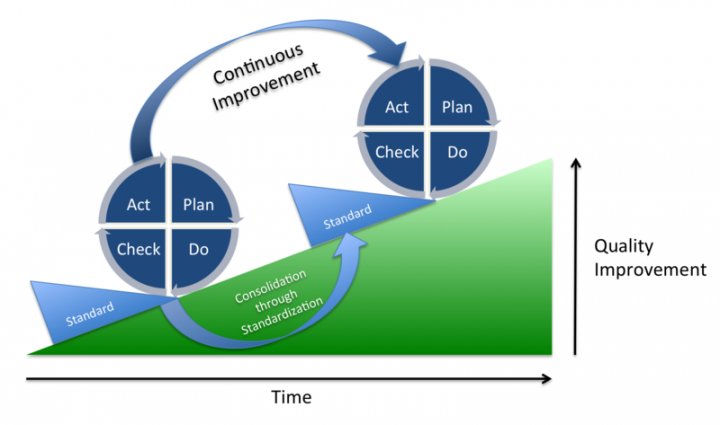
\includegraphics[width=0.85\textwidth]{images/pdca.png}
    \caption{\acrlong{pdca}}
    \captionsetup{aboveskip=2pt}
    \caption*{\begin{footnotesize}\textit{Fonte:} \url{http://quickstart-indonesia.com/siklus-pdca/}\end{footnotesize}}
  \end{center}
\end{figure}

L'adozione del \sacrfoot{pdca} (figura \thefigure) nel mio metodo di lavoro è stato essenziale per dei miglioramenti personali in diversi ambiti, soprattutto quelli legati alla gestione del tempo (come visto nella sotto-sezione \ref{subsub:auto-miglioramento}), efficienza organizzativa ed efficacia di sviluppo.

Ritengo dunque di aver raggiunto tutti gli obiettivi personali posti, con risultati addirittura migliori delle mie aspettative iniziali.

\section{Distanza rispetto ai contenuti del corso di studi}

Nonostante le tecnologie e i concetti utilizzati nel percorso siano stati per me una novità rispetto agli insegnamenti previsti nel Corso di Laurea, \textbf{ritengo che il percorso di studi abbia completamente soddisfatto i requisiti necessari per il completamento dello \stage.}

Infatti, sebbene gli insegnamenti non abbiano specificatamente trattato le moderne tecnologie utilizzate, mi hanno fornito la preparazione necessaria al loro  rapido apprendimento; in un settore lavorativo in rapida evoluzione come quello dell'informatica, la capacità di adattamento all'utilizzo di strumenti moderni come Apache Kafka e quella di comprendere facilmente le architetture innovative è di fondamentale importanza e personalmente molto apprezzata.

% Alcuni corsi in particolare hanno provveduto sostanzialmente la distanza tra l'ambiente universitario e quello lavorativo, quali ingegneria del software (con progetto associato), basi di dati, tecnologie web, e i vari corsi di programmazione.
Mi ritengo pertanto pienamente soddisfatto del percorso di studi e soprattutto del percorso di \stage; ritengo essi abbiano dato una rapida accelerazione alla mia formazione professionale e abbia fornito i presupposti necessari per un mio inserimento nell'ambiente lavorativo.


% TODO: In §4.4 non menzionerai specifici insegnamenti, neanche in positivo, ma ragionerai sul complesso del percorso di studi.
